\section{Oscilador Harmônico Simples}

\subsection{Movimento Periódico}

Um movimento é dito periódico quando um objeto saí de uma posição e, após um certo intervalo de tempo chamado Período ($T$), retorna a essa posição original com a mesma velocidade. Matematicamente falando:

\[ \large \vec{r}(t + T) = \vec{r}(t)\]

\[ \large \vec{v}(t + T) = \vec{v}(t)\]

Onde $\vec{r}$ e $\vec{v}$ são respectivamente os vetores posição e velocidade deste objeto.  
Outra característica importante de um movimento periódico é a frequência ($f$) que representa o número de vezes que o movimento se repete em uma unidade de tempo. Tal propriedade é definida como sendo o inverso do Período:

\[\Large f = \frac{1}{T}\]

\subsection{Força elástica}

É a força que proporciona o movimento periódico. As vezes denominada força restauradora, esta tende a restaurar o equilíbrio retornando o objeto a posição de equilíbrio toda vez que o mesmo é deslocado. Esse tipo de força tem a forma semelhante a:

\[ \large F = -kx\]

A variável $k$ representa a constante elástica da mola, e é especifica para o material que compõe a mola.

\subsection{Equação do movimento}

Pela segunda lei de newton, sabemos que a força resultante sobre um objeto é igual ao produto da massa pela aceleração deste.  Podemos determinar uma equação que descreva a posição de um objeto em função do tempo, a partir da segunda lei de newton. Imagine um corpo qualquer de massa $m$ preso a uma mola de constante elástica $k$, como na figura abaixo.

\begin{figure}[H]
	\centering
	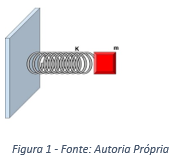
\includegraphics[width=0.5\textwidth]{./Imagens/OHS/ohs1.png} 
	\caption{Sistema massa-mola}
	\label{fig:OHS1}
\end{figure}

Considerando que a força aplicada a esse corpo de massa $m$, seja a força restauradora mencionada acima, temos que:

\[\Large ma = -kx\]

Podemos escrever a aceleração $a$ como sendo a segunda derivada em relação ao tempo t. Sendo assim, a equação acima fica: 

\[\Large m \frac{d^2x(t)}{dt^2} = -kx(t)\]

Temos em mãos, então, uma equação diferencial ordinária (EDO) que delimita a posição de um oscilador harmônico simples (OHS) em função do tempo.

Para determinarmos a expressão da função $x(t)$, precisamos resolver essa equação acima.  O intuito do presente trabalho é utilizar computação numérica, com a linguagem Scilab para isso. 

Antes de tudo é necessário utilizar um artificio matemático para transformar a EDO de 2ª ordem acima, em um sistema de 2 EDO’s de 1ª ordem. Para isso, fazemos: 

\[\Large \frac{dx(t)}{dt} = v\]

Dessa forma, fica implícito que:

\[\Large \frac{dv}{dt} = \frac{d^2x(t)}{dt^2}\]

Portanto, fazendo as devidas substituições temos o seguinte sistema:

\[\Large \frac{dx(t)}{dt} = v\]

\[\Large \frac{dv}{dt} = -\frac{k}{m}x(t)\]

Com isso aplicamos o método numérico de Euler para o sistema acima:

\begin{minted}{Scilab}
//Resolução da equação de movimento para OHS
//A equação é: X''(t) = -(k/m)X(t) uma edo de 2ª ordem

//Parâmetros do problema
//m = 1kg; K = 1N/m; 
//Intervalo de tempo  = 0 à 40 segundos 
// deslocamento da mola incialmente é 0.20 metros
// velocidade no instante t = 0 é 0 metros/segundo

clear,clc
// definindo o intervalo de tempo
t0 = input("informe o valor inicial do intervalo: ");
tn = input("informe o valor final do intervalo: ");
h = input("Informe o passo h: ");
t = t0:h:tn // criando o vetor intervalo de tempo
t = t' // apenas transpoe o vetor t
k = input("informe a constante da mola:")
m = input("informe a massa do objeto: ")

//condições iniciais
// objeto deslocado 0.20 m da posição de equilibrio
w1(1) = 0.20 
// no instante que o objeto é solto, 
// têm se velocidade igual a zero
w2(1) = 0 

for j = 2:length(t)
w1(j) = w1(j-1) + w2(j-1)*h //diz respeito a X(t)
w2(j) = w2(j-1) -(k/m)*w1(j-1)*h // diz respeito a V(t)
end
// determinado para o caso especifico 
// de m = 1kg, k = 1N/m, X(0) = 0.20m, theta_inicial  = 0
function x = f(t)
//w1(1) corresponde ao deslocamento inicial da mola
x = w1(1)*cos(sqrt(k/m)*t) 
endfunction
plot2d(t,[w1, f()], leg = "Numérico@Exata@")
\end{minted}